
\chapter{Ambisonics}
\label{chap:ambisonics}

%-----------------------------------------------
%   INTRODUCTION
%-----------------------------------------------

\lettrine{T}{he} Ambisonics format is an audio format capable of efficiently representing the spatial aspect of a sound field. Hence, it has become a popular format for 3D spatial audio coding \cite{pulkki_parametric_2018}, as a \emph{de facto} standard in both professional and consumer domains \cite{herre_mpeg-h_2014} (see also the Facebook 360\footnote{https://facebook360.fb.com/spatial-workstation/} and the Google360\footnote{https://support.google.com/youtube/answer/6395969} systems available online).
Ambisonics finds its roots in the 1930s, when Blumlein's original work \cite{blumlein_improvements_1931} on coincident stereo recordings proposed to place two figure-of-eight microphones in a orthogonal manner. Gerzon \cite{gerzon_periphony_1973} extended this idea in the 1970s by theorizing what we call the first-order Ambisonics (FOA) format, originally known as B-format, which paved the path to high-order Ambisonics (HOA) \cite{daniel_representation_2001}.

While the term Ambisonics arose from the design of the corresponding microphones, we also often encounter terms related to the spherical harmonics theory in the literature. In fact, the Ambisonics representation consists of the coefficient of the spherical harmonics decomposition of the signal. In this thesis, we will use the term Ambisonics because of the past of the laboratory we conducted our research in, but in this chapter we show how both theories are linked together.

In this chapter, we establish the theoretical foundations of the Ambisonics format, which we adopted to represent audio signals in this thesis. After briefly explaining why this format is of interest, we derive the spherical harmonics decomposition of the solution of the wave equation. This decomposition leads us to the definition of first-order and higher-order Ambisonics. We finally discuss several representations derived from the Ambisonics format, useful for sound scene analysis: the pseudointensity vector, the frequency-domain velocity vector, and the time-domain velocity vector.

An interesting reader may find more in-depth details in diverse references, \emph{e.g.}, theses \cite{daniel_representation_2001,merimaa_analysis_2006,baque_analyse_2017,moreau_etude_2006}, or books \cite{zotter_ambisonics_2019, rafaely_fundamentals_2019, jarrett_theory_2017, williams_fourier_2000}.

%-----------------------------------------------
%   INTEREST OF THE AMBISONICS FORMAT
%-----------------------------------------------
\section{Interest of the Ambisonics format}

One of the main benefits of the Ambisonics lies in its capability of compactly encoding the surrounding sound scene in a format that is theoretically agnostic regarding the configuration of the recording microphone array. Likewise, the Ambisonics format is flexible with respect to the setup of an audio system used for reproduction, as its decoding can be adapted to match the given layout, \emph{e.g.}, to headphones, stereo monitors, 5.1 audio systems, or even a setup with many loudspeakers \cite{zotter_ambisonics_2019}. The Ambisonics format is an isotropic representation of the sound field, \emph{i.e.}, the encoding takes equally into account all spatial directions. It contains the directional information of the sound sources, due to the microphones nature and orientation. A particularity of this characteristics is that it becomes very handy to perform some transformations of the encoded sound recording: for instance, one can easily rotate the sound field by multiplying the multi-channel recording by the appropriate matrix. One typical application of such a property is to take into account the movement of a robot's head when localizing surrounding sounds.

Due to these advantages, more and more commercial applications opt for this sound representation to handle audio signals. As we have seen above, internet giants such as Google or Facebook use the Ambisonics format for their spatial audio applications, especially in virtual reality (VR) environments. Recently, we have witnessed an increase of available easy-to-use devices that can be used to record spatial audio in the Ambisonics format (see Fig.~\ref{fig:ambisonics_microphones}): mh acoustics' EigenMike,\footnote{https://mhacoustics.com/products\#eigenmike1} Zoom's H3-VR recorder,\footnote{https://zoomcorp.com/fr/fr/enregistreurs-portatifs/handheld-recorders/h3-vr-360-audio-recorder/} Zylia's ZM-1.\footnote{https://www.zylia.co/zylia-zm-1-microphone.html} Decoding tools are also largely available nowadays, especially to be used in digital audio workstations (DAW): IEM plug-in suite,\footnote{https://plugins.iem.at/} b<>com plug-ins,\footnote{https://b-com.com/en/process/spatial-audio-family} IRCAM's Panoramix,\footnote{https://forum.ircam.fr/projects/detail/panoramix/} or Noise Makers' Ambi Head HD\footnote{https://www.noisemakers.fr/ambi-head-hd/} to name a few.

\begin{figure}[t]
    \begin{center}
    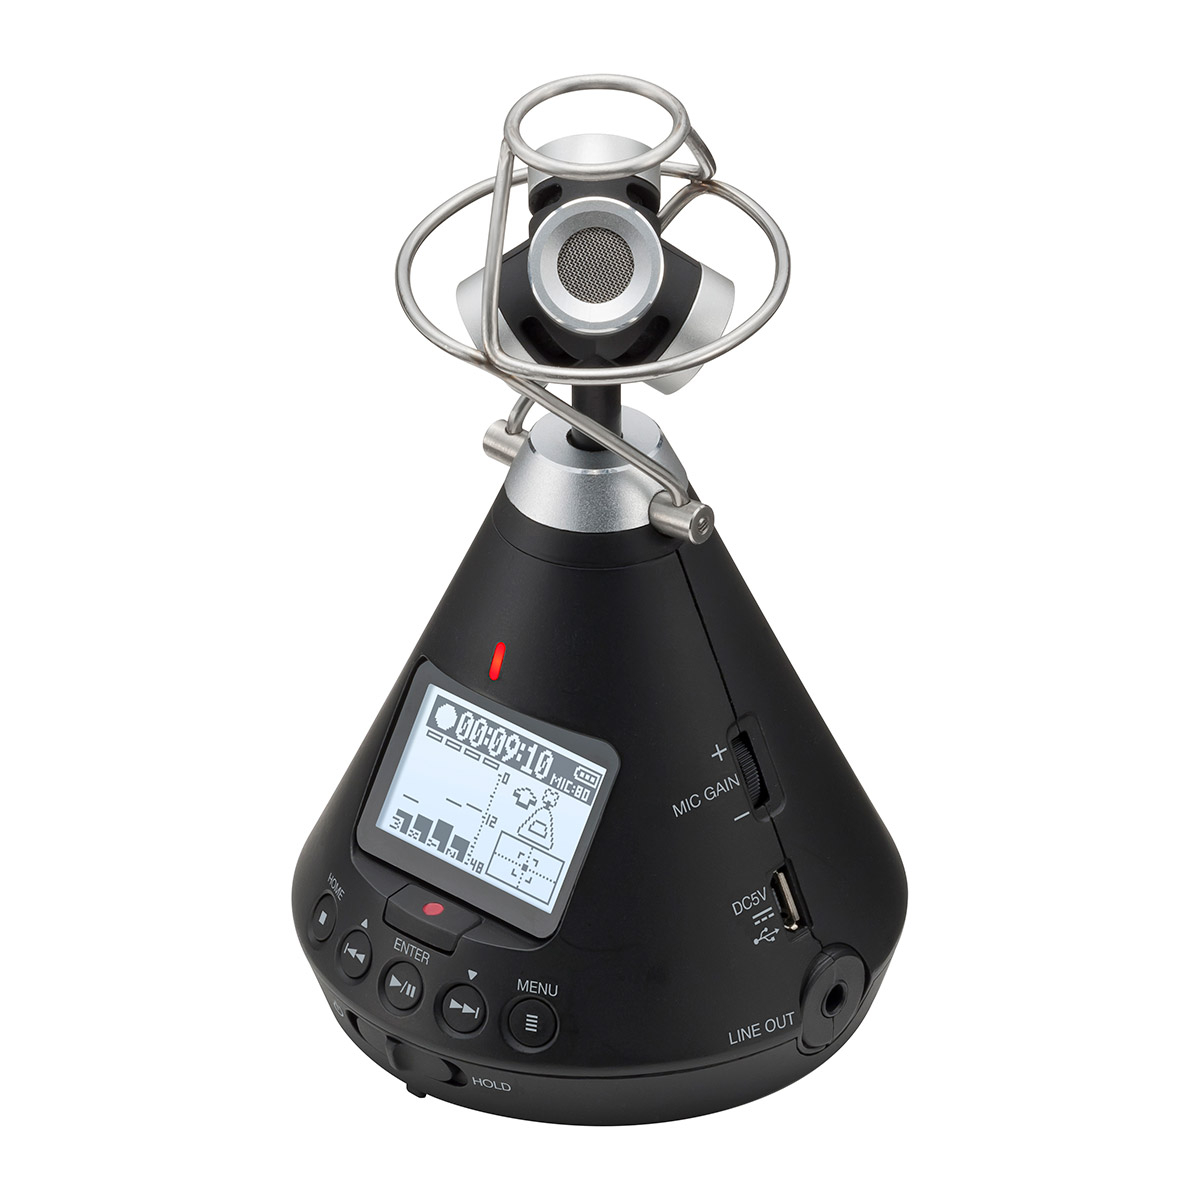
\includegraphics[width=0.35\linewidth]{Images/chap2/h3-vr.jpg}
    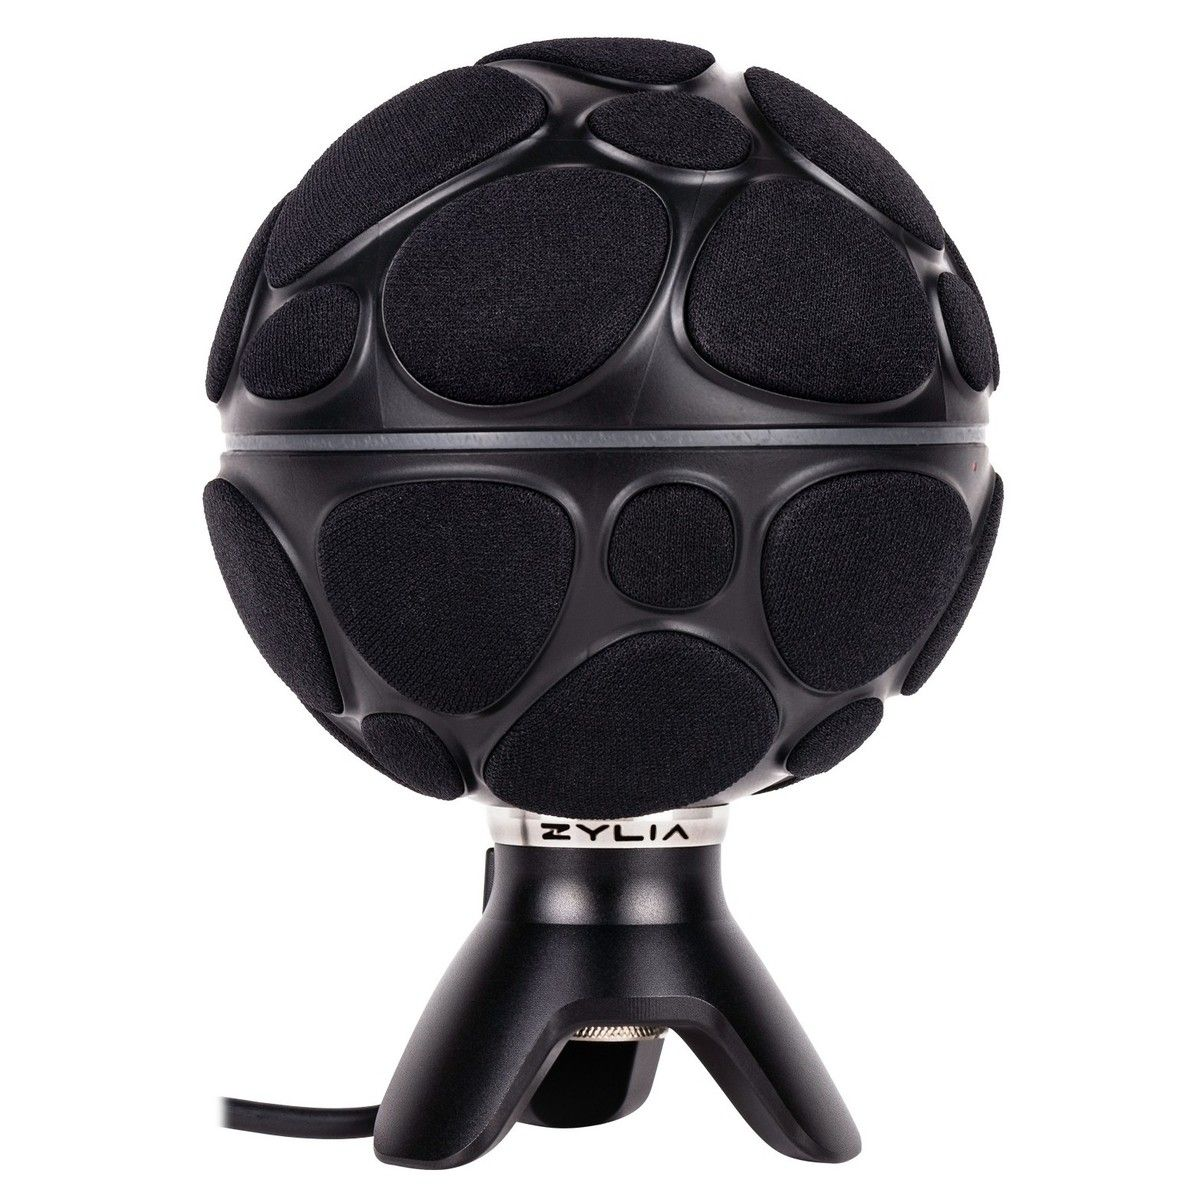
\includegraphics[width=0.35\linewidth]{Images/chap2/zm-1.jpg}
    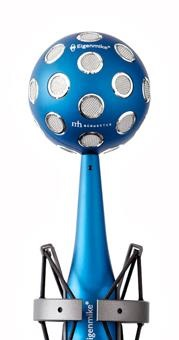
\includegraphics[width=0.2\linewidth]{Images/chap2/eigenmike.jpg}
    \captionof{figure}[Examples of Ambisonics microphone arrays]{Examples of microphone arrays suitable for the encoding of the recorded sound field into the Ambisonics format. \textbf{Left}: Zoom's H3-VR (4 capsules, Ambisonics format up to order 1); \textbf{middle}: Zylia's ZM-1 (19 capsules, up to order 3); \textbf{right}: mh acoustics' EigenMike (32 capsules, up to order 4).}
    \label{fig:ambisonics_microphones}
    \end{center}
\end{figure}

%-----------------------------------------------
%   WAVE EQUATION AND SHD
%-----------------------------------------------
\section{Wave equation and spherical harmonics decomposition}

In this section, we derive the solution of the wave equation in the spherical domain and exhibit the spherical harmonics decomposition of the sound signal, which will lead to the definition of the Ambisonics format in the section~\ref{sec:ambisonics}.

\subsection{Wave equation solution in the spherical domain}

A sound signal is the evolution of the sound pressure $p(\mathbf{r},t)$ with time $t$ at the recording point $\mathbf{r}$, which is measured in Pascals (Pa). The recorded signal is due to the sound source which produces a sound wave, \emph{i.e.}, the solution of the famous \textit{acoustic wave equation} :
\begin{equation}
\label{eq:waveEquation}
    \nabla^2 p(\mathbf{r},t) - \frac{1}{c^2} \frac{\partial^2}{\partial t^2} p(\mathbf{r},t) = 0,
\end{equation}
where $\nabla^2$ denotes the Laplacian operator and $c$ is the speed of sound in the considered fluid (in the air, $c = \SI{343}{\meter\per\second}$ at $\SI{20}{\degreeCelsius}$).

We want to find the general solution of the wave equation in the three-dimensional space. To do that, we represent the 3D space using spherical coordinates, \emph{i.e.}, ${\mathbf{r} = (r, \theta, \phi)}$, where $\theta$ is the azimuth angle and $\phi$ the elevation angle, as illustrated in Fig.~\ref{fig:spherical_coordinates}. The following equations describe the relationship between cartesian and spherical coordinates:
\begin{equation}
\label{eq:spherical_coordinates}
    \left\{ 
    \begin{aligned} 
      x &= r \cos\theta \cos\phi \\
      y &= r \sin\theta \cos\phi. \\
      z &= r \sin\phi
    \end{aligned}
    \right.
\end{equation}

\begin{figure}[t]
    \begin{center}
    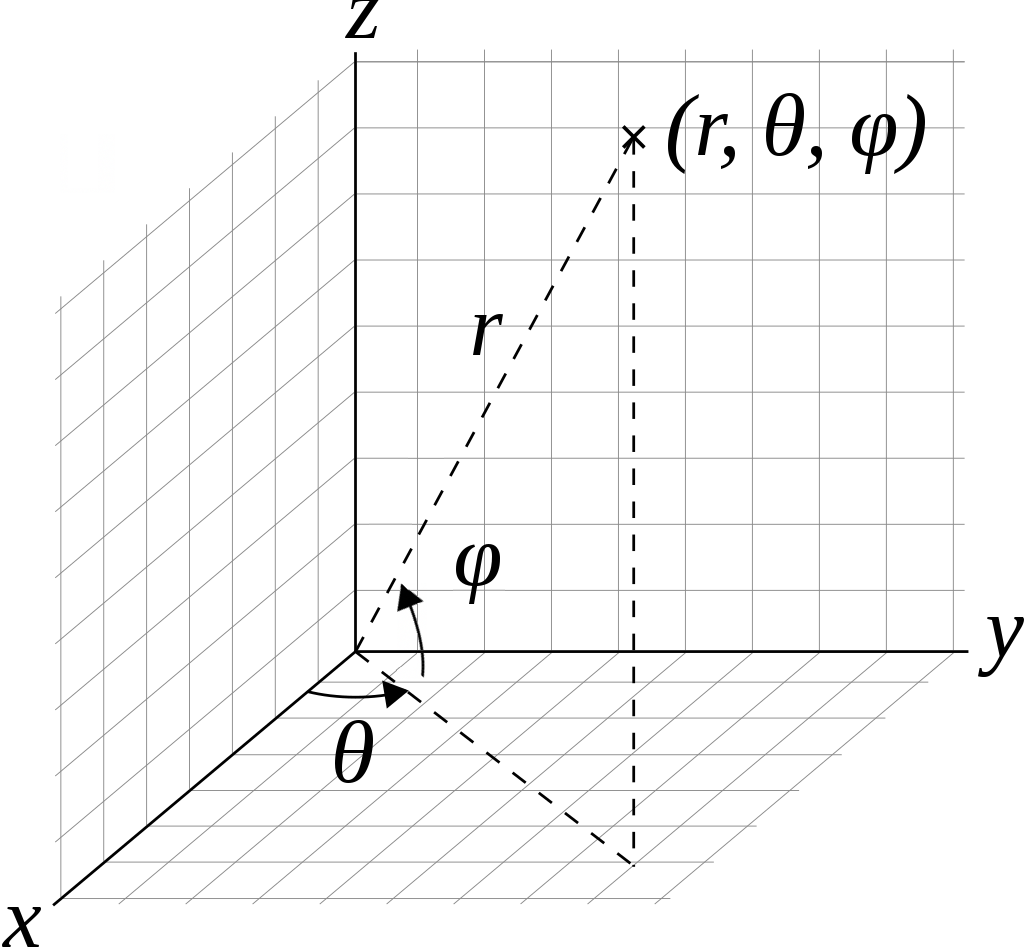
\includegraphics[width=0.4\linewidth]{Images/chap2/spherical_coordinates.png}
    \captionof{figure}[Spherical coordinate system]{Spherical coordinate system. Any position in space can be described with three numbers: the distance $r$, the azimuth angle $\theta$ and the elevation angle (or polar angle) $\phi$. The relation between spherical coordinates $r,\theta, \phi$ and cartesian coordinates $x,y,z$ is given by \eqref{eq:spherical_coordinates}. Borrowed from \href{https://commons.wikimedia.org/wiki/File:3D_Spherical_2.svg}{Dmcq, CC BY-SA 3.0}.}
    \label{fig:spherical_coordinates}
    \end{center}
\end{figure}

In three dimensions, using spherical coordinates, the Laplacian operator for a function $f(r,\theta,\phi)$ is given by:
\begin{equation}
\label{eq:sphericalLaplacian}
    \nabla_\mathbf{r}^2 f = \frac{1}{r^2} \frac{\partial}{\partial r} \bigg(r^2 \frac{\partial f}{\partial r} \bigg) + \frac{1}{r^2 \sin\theta} \frac{\partial}{\partial \theta} \bigg(\sin\theta \frac{\partial f}{\partial \theta} \bigg) + \frac{1}{r^2 \sin^2 \theta} \frac{\partial^2 f}{\partial \phi^2}.
\end{equation}

To derive a solution for the wave equation in the spherical domain, one can proceed to a separation of variables, \emph{i.e.}, we assume that $p$ takes the form:
\begin{equation}
    \label{eq:separationVariables}
    p(r,\theta,\phi,t) = R(r)\Theta(\theta)\Phi(\phi)T(t).
\end{equation}
Then, by injecting \eqref{eq:separationVariables} in \eqref{eq:waveEquation} using \eqref{eq:sphericalLaplacian}, we obtain one separate partial equation for each variable $r$, $\theta$, $\phi$ and $t$ \cite[p.~35]{rafaely_fundamentals_2019}:
\begin{equation}
\label{eq:partialEquationR}
    r^2 \frac{d^2}{dr^2} R + 2r \frac{d}{dr} R + \big[(kr)^2 - n(n+1)\big] R = 0,
\end{equation}
with $k=\frac{\omega}{c}$ being the wave number of the sound wave ($\omega = 2 \pi f$ is the angular frequency),
\begin{equation}
\label{eq:partialEquationTheta}
      \frac{d}{d \mu} \bigg[(1-\mu^2)\frac{d}{d \mu} \Theta \bigg] + \bigg[n(n+1) - \frac{m^2}{1-\mu^2} \bigg] \Theta = 0,
\end{equation}
with $\mu = \cos^2 \theta$ and $\lvert m \rvert \leq n, m \in \mathbb{Z}, \; n \in \mathbb{N}$,
\begin{equation}
\label{eq:partialEquationPhi}
      \frac{d^2 \Phi}{d \phi^2} + m^2 \Phi = 0,
\end{equation}
and
\begin{equation}
\label{eq:partialEquationT}
      \frac{d^2 T}{dt^2} + \omega^2 T = 0, \quad \omega \in \mathbb{R}.
\end{equation}
\eqref{eq:partialEquationPhi} and \eqref{eq:partialEquationT} immediately lead to the following exponential solutions, valid for an harmonic wave, \emph{i.e.}, with a single frequency $\omega$ :
\begin{equation}
    T(t) = e^{i \omega t},
\end{equation}
and 
\begin{equation}
    \Phi(\phi) = e^{i m \phi},
\end{equation}
where $i = \sqrt{-1}$. Note that $m$ is an integer because $\Phi$ is $2 \pi$-periodic.
\eqref{eq:partialEquationTheta} is known as the associated \textit{Legendre differential equation}, whose non-singular solutions are given by the associated \textit{Legendre functions of the first kind} \cite[p.~715]{arfken_mathematical_2013}:
\begin{equation}
    \Theta(\theta) = P_n^m(\cos\theta), \quad m \in \mathbb{Z}, n \in \mathbb{N}.
\end{equation}
\eqref{eq:partialEquationR} is referred as the \textit{spherical Bessel equation}, whose solutions are a weighted combination of the \textit{spherical Bessel functions of the first kind} $j_n(kr)$ and the \textit{spherical Hankel functions of the first kind} $h_n(kr)$:
\begin{equation}
    R(r) = R_1 j_n(kr) + R_2 h_n(kr),
\end{equation}
with $R_1$, $R_2 \in \mathbb{R}$. In fact, in our case, we have necessarily $R_2=0$ since the functions $h_n$ diverge at $r=0$ and we suppose that no infinite sound pressure occurs at the recording point.

Finally, combining these variable-wise equations leads to the set of fundamental solutions for the wave equation in the spherical domain :
\begin{equation}
\label{eq:solutionWaveEquation}
    p(\mathbf{r},t) = R_1 j_n(kr) P_n^m(\cos \theta) e^{im\phi} e^{iwt},
\end{equation}
with $n \in \mathbb{N}$, $m \in \mathbb{Z}$ and $\lvert m \rvert \leq n$. The general solution is a weighted sum of these fundamental solutions. The products formed by the angular factors $P_n^m(\cos \theta)$ and $e^{im\phi}$ are known to be the (scaled) \textit{spherical harmonics}, which brings us to the next subsection.

\subsection{Spherical harmonics}

\subsubsection{Complex spherical harmonics}

The terms depending on $\theta$ and $\phi$ on the wave equation solutions \eqref{eq:solutionWaveEquation} are grouped together to define the complex spherical harmonics. This set of complex functions, indexed by $n$ and $m$, are defined on the unit sphere by \cite[p.~4]{rafaely_fundamentals_2019}:
\begin{equation}
    Y_n^m(\theta,\phi) = \sqrt{\frac{2n+1}{4 \pi} \frac{(n-m)!}{(n+m)!}} P_n^m(\cos\theta) e^{i m \phi},
\end{equation}
where $n \in \mathbb{N}$ is the order, and $m \in \{-n, -n+1, ..., n-1, n\}$ is the degree of the spherical harmonic. We recognize the associated Legendre functions as well as the exponential function of the elevation $\phi$.

An interesting property of these complex spherical harmonics is that they form an orthonormal basis of the Hilbert space $L_2(S^2)$ (\emph{i.e.}, the set of all square-integrable complex functions of the unit sphere), with the following inner product:
\begin{equation}
    \langle f \mid g \rangle = \frac{1}{4 \pi} \int_{\theta=0}^{2 \pi} \int_{\phi=-\frac{\pi}{2}}^{\frac{\pi}{2}} f(\theta,\phi) g(\theta,\phi)^* \cos \phi d \phi d \theta,
\end{equation}
where $*$ denotes the complex conjugates.
This property involves that any function $f(\theta,\phi)\in L_2(S^2)$ can be decomposed as a weighted sum of spherical harmonics:
\begin{equation}
    f(\theta,\phi) = \sum_{n=0}^{\infty} \sum_{m=-n}^{n} f_{nm} Y_n^m(\theta,\phi),
\end{equation}
with $f_{nm}$ denoting the coefficients of $f(\theta,\phi)$ on this basis. This representation is known as the \textit{spherical harmonics decomposition} (SHD) of $f(\theta,\phi)$. The coefficients $f_{nm}$ can be computed as:
\begin{equation}
    \begin{split}
    f_{nm} &= \langle f(\theta,\phi) \mid Y_n^m(\theta,\phi) \rangle \\
           &= \int_{\theta=0}^{2 \pi} \int_{\phi=-\frac{\pi}{2}}^{\frac{\pi}{2}} f(\theta,\phi) Y_n^m(\theta,\phi)^* \cos\phi d \phi d \theta.
    \end{split}
\end{equation}

From \eqref{eq:solutionWaveEquation}, we can express the general solution (linear sum of fundamental solutions) of the wave equation on the basis of spherical harmonics:
\begin{equation}\label{eqHOAdecomp}
    p(\theta,\phi,r,t) = \sum_{n=0}^{\infty} \sum_{m=-n}^n \alpha_{nm} j_n(kr) Y_n^m(\theta,\phi) e^{i \omega t},
\end{equation}
where $\alpha_{nm} \in \mathbb{R}$ are the weights of each fundamental solution. 

\subsubsection{Real spherical harmonics}
\label{sec:realSphericalHarmonics}

\textit{Real} spherical harmonics $\tilde{Y}_n^m$ also exist and are defined by \cite[p.~28]{jarrett_theory_2017}:
\begin{equation}
\label{eq:realSphericalHarmonicsDefinition}
    \tilde{Y}_n^m(\theta,\phi) = (-1)^{\lvert m \rvert} \sqrt{\frac{2n+1}{4 \pi} \frac{(l-\lvert m \rvert)!}{(l+\lvert m \rvert)!}} P_n^{\lvert m \rvert}(\cos\theta) 
    \begin{cases}
        \sqrt{2} \sin(\lvert m \rvert \phi), & \text{if $m<0$}\\
        1, & \text{if $m=0$}. \\
        \sqrt{2} \cos(m \phi), & \text{if $m>0$}\\
    \end{cases}
\end{equation}

The real spherical harmonics $\tilde{Y}_n^m$ can be derived from the complex spherical harmonics by:
\begin{equation}
    \tilde{Y}_n^m(\theta,\phi) = 
    \begin{cases}
        \sqrt{2} (-1)^m \mathfrak{I} (Y_n^{-m}(\theta,\phi)), & \text{if $m<0$} \\
        Y_n^0(\theta,\phi), & \text{if $m=0$}, \\
        \sqrt{2} (-1)^m \mathfrak{R} (Y_n^m(\theta,\phi)), & \text{if $m>0$}
    \end{cases}
\end{equation}
where $\mathfrak{R}(\cdot)$ and $\mathfrak{I}(\cdot)$ denote the real and imaginary parts of the argument, respectively.
Inversely, the complex spherical harmonics $Y_n^m$ can be obtained from the real spherical harmonics:
\begin{equation}
\label{eq:real2complex}
    Y_n^m(\theta,\phi) = 
    \begin{cases}
        \frac{1}{\sqrt{2}} (\tilde{Y}_n^{-m}(\theta,\phi) - i \tilde{Y}_n^m(\theta,\phi)), & \text{if $m<0$} \\
        \tilde{Y}_n^0(\theta,\phi), & \text{if $m=0$}. \\
        \frac{1}{\sqrt{2}} (-1)^m (\tilde{Y}_n^m(\theta,\phi) + i \tilde{Y}_n^{-m}(\theta,\phi)), & \text{if $m>0$}
    \end{cases}
\end{equation}
The real-valued spherical harmonics also form an orthogonal basis of the set of real functions on the unit sphere, using the inner product \cite[p.~302]{daniel_representation_2001}:
\begin{equation}
    \langle f \mid g \rangle = \frac{1}{4 \pi} \int_{\theta=0}^{2 \pi} \int_{\phi=-\frac{\pi}{2}}^{\frac{\pi}{2}} f(\theta,\phi) g(\theta,\phi) \sin \phi d \phi d \theta.
\end{equation}

An orthonormal basis can be defined by scaling each real spherical harmonic $\tilde{Y}_n^m$ by $\sqrt{2n+1}$ \cite{daniel_representation_2001}, and similarly to the complex spherical harmonics, we can decompose any real function $f(\theta,\phi)$ on the unit sphere on this basis:
\begin{equation}\label{eqHOArealDecomp}
    f(\theta,\phi) = \sum_{n=0}^\infty \sum_{m=-n}^{n} f_{nm} \tilde{Y}_n^m(\theta,\phi),
\end{equation}
where $f_{nm}$ are the coefficients of the decomposition.

\subsection{Wave equation solution for a single plane wave}

To define the Ambisonics components from the wave equation solution, we focus on deriving the solution for a single plane wave, and then we deduce the expression in the general case. We consider a single-frequency plane wave arriving from direction $(\theta_k,\phi_k)$, with amplitude $B$ and wave number $k=\frac{\omega}{c}$, $\omega = 2 \pi f$ where $f$ is the frequency of the wave. This plane wave also satisfies the general solution of the wave equation, and it can be shown that in this case the solution can be written as \cite[p.~227]{williams_fourier_2000}:
\begin{equation}
    p(r,\theta,\phi,t) = 4 \pi B e^{i \omega t} \sum_{n=0}^{\infty}  i^n  j_n(kr) \sum_{m=-n}^n Y_n^m(\theta,\phi) Y_n^m(\theta_k,\phi_k)^*.
\end{equation}

Using the relation between real and complex spherical harmonics in \eqref{eq:real2complex}, we can express the sum containing complex spherical harmonics in terms of real spherical harmonics:
\begin{equation}
    \sum_{m=-n}^n Y_n^m(\theta,\phi) Y_n^m(\theta_k,\phi_k)^* = \sum_{m=-n}^n \tilde{Y}_n^m(\theta,\phi) \tilde{Y}_n^m(\theta_k,\phi_k),
\end{equation}
leading to the expression of the pressure for the single plane wave, using real spherical harmonics:
\begin{equation}
\label{eq:planeWaveDecomposition}
    p(r,\theta,\phi,t) = B e^{i \omega t} \sum_{n=0}^{\infty}  i^n  j_n(kr) \sum_{m=-n}^n \tilde{Y}_n^m(\theta,\phi) \tilde{Y}_n^m(\theta_k,\phi_k),
\end{equation}
where the constant term $4 \pi$ has been incorporated in the amplitude term $B$. This last expression for the solution of the wave equation in the spherical domain (for a single plane wave) brings us to the definition of the Ambisonics coefficients.
%-----------------------------------------------
%   FOA & HOA
%-----------------------------------------------

\section{First-order and higher-order Ambisonics}
\label{sec:ambisonics}

\subsection{Definition of Ambisonics coefficients}

\eqref{eq:planeWaveDecomposition} exhibits a solution of the wave equation for a single-frequency plane wave of amplitude $A$, angular frequency $\omega$ and coming from direction $(\theta_k,\phi_k)$. The Ambisonics coefficients are defined as the coefficients of the decomposition of the pressure $p$ on the basis of real spherical harmonics \cite{daniel_representation_2001}:
\begin{equation}\label{eqPlaneWaveCf}
    B_n^m(t) = B e^{i \omega t} \tilde{Y}_n^m (\theta_k,\phi_k).
\end{equation}
As we can see, the propagation term $i^n j_n(kr)$ is not taken into account when deriving the Ambisonics components. In fact, this term can be computed for all $r$, so a sound field can be completely recreated based on the Ambisonics coefficients only.

Finally, the definition of Ambisonics coefficients can be extended to the general case of a composite point source signal $s(t)$ with different frequencies (\emph{i.e.}, not only a single-frequency wave):
\begin{equation}\label{eqPlaneWaveCoeff}
     B_n^m(t) = s(t) \tilde{Y}_n^m(\theta_k,\phi_k).
 \end{equation}
 
\eqref{eq:planeWaveDecomposition} and \eqref{eqHOAdecomp} state that we can represent the sound field at any given point in space using the infinite number of Ambisonics coefficients. In practice, the number of available Ambisonics coefficients is limited (we explain why in subsection~\ref{subAmbEncoding}). Hence, the infinite summation over $n$ is truncated up to the \textit{Ambisonics order} $N$ :
\begin{equation}\label{eqAmbiDecomp}
    p(r,\theta,\phi,t) \approx \sum_{n=0}^{N}  i^n  j_n(kr) \sum_{m=-n}^n  B_n^m(t) \tilde{Y}_n^m(\theta,\phi).
\end{equation}
The truncation above restricts the set of functions $p$ that can be faithfully represented by such a reduced set of coefficients. Therefore, we assume that $p$ is ``order-limited'', \emph{i.e.}, that its expansion coefficients for the orders higher than $N$ are negligible \cite{rafaely_fundamentals_2019} (this is analogous to band-limited functions in classical Fourier analysis). Such functions can be spatially sampled, and perfectly reconstructed, from $(N+1)^2$ nearly-uniform measurements on the sphere \cite{jarrett_theory_2017}.


\subsection{First-order Ambisonics}

When $N=1$, the truncated representation of $p$ is called \textit{first-order Ambisonics}. It has been originally proposed by Gerzon \cite{gerzon_periphony_1973} in the 1970s, who referred to it as the \textit{B-format}. This representation includes four components: $B_0^0$ for $n=0$, usually written as $W$, and $B_1^1$, $B_1^{-1}$ and $B_1^0$ for $n=1$, usually written as $X$, $Y$ and $Z$, respectively. The choice of designation for $X$, $Y$ and $Z$ follows the directivity of the spherical harmonics according to the usual axes $x,y,z$ of an Euclidean space. For a plane wave coming from $(\theta_k,\phi_k)$ and carrying a signal $s(t)$, the FOA representation is obtained using \eqref{eq:realSphericalHarmonicsDefinition}:\footnote{In this thesis we use the N3D normalization standard \cite{daniel_representation_2001}, which makes use of the real spherical harmonics normalized with $\sqrt{2n+1}$ as introduced in Sec.~\ref{sec:realSphericalHarmonics}.}
\begin{equation}\label{eqPlaneWave}
\mathbf{x}(t) = 
\begin{bmatrix} W(t) \\ X(t) \\ Y(t) \\ Z(t) \end{bmatrix}
= \begin{bmatrix} s(t) \tilde{Y}_0^0(\theta_k,\phi_k) \\ s(t) \tilde{Y}_1^1(\theta_k,\phi_k) \\ s(t) \tilde{Y}_1^{-1}(\theta_k,\phi_k) \\ s(t) \tilde{Y}_1^0(\theta_k,\phi_k) \end{bmatrix}
= \begin{bmatrix} 1 \\ \sqrt{3} \cos \theta_k \cos \phi_k \\ \sqrt{3} \sin \theta_k \cos \phi_k \\ \sqrt{3} \sin \phi_k \end{bmatrix} s(t).
\end{equation}
The directivities of the FOA components are illustrated on Fig.~\ref{fig:foa}. We can interpret these four components as the recordings of four spatially coincident microphones: $W$ represents the recording of an omnidirectional microphone, and $X$, $Y$ and $Z$ represent the recordings of three bidirectional microphones, each oriented on the corresponding axis. The channels $X$, $Y$ and $Z$ are assimilated to pressure gradients, which will be a useful propriety later in this chapter.

\begin{figure}[t]
    \begin{center}
    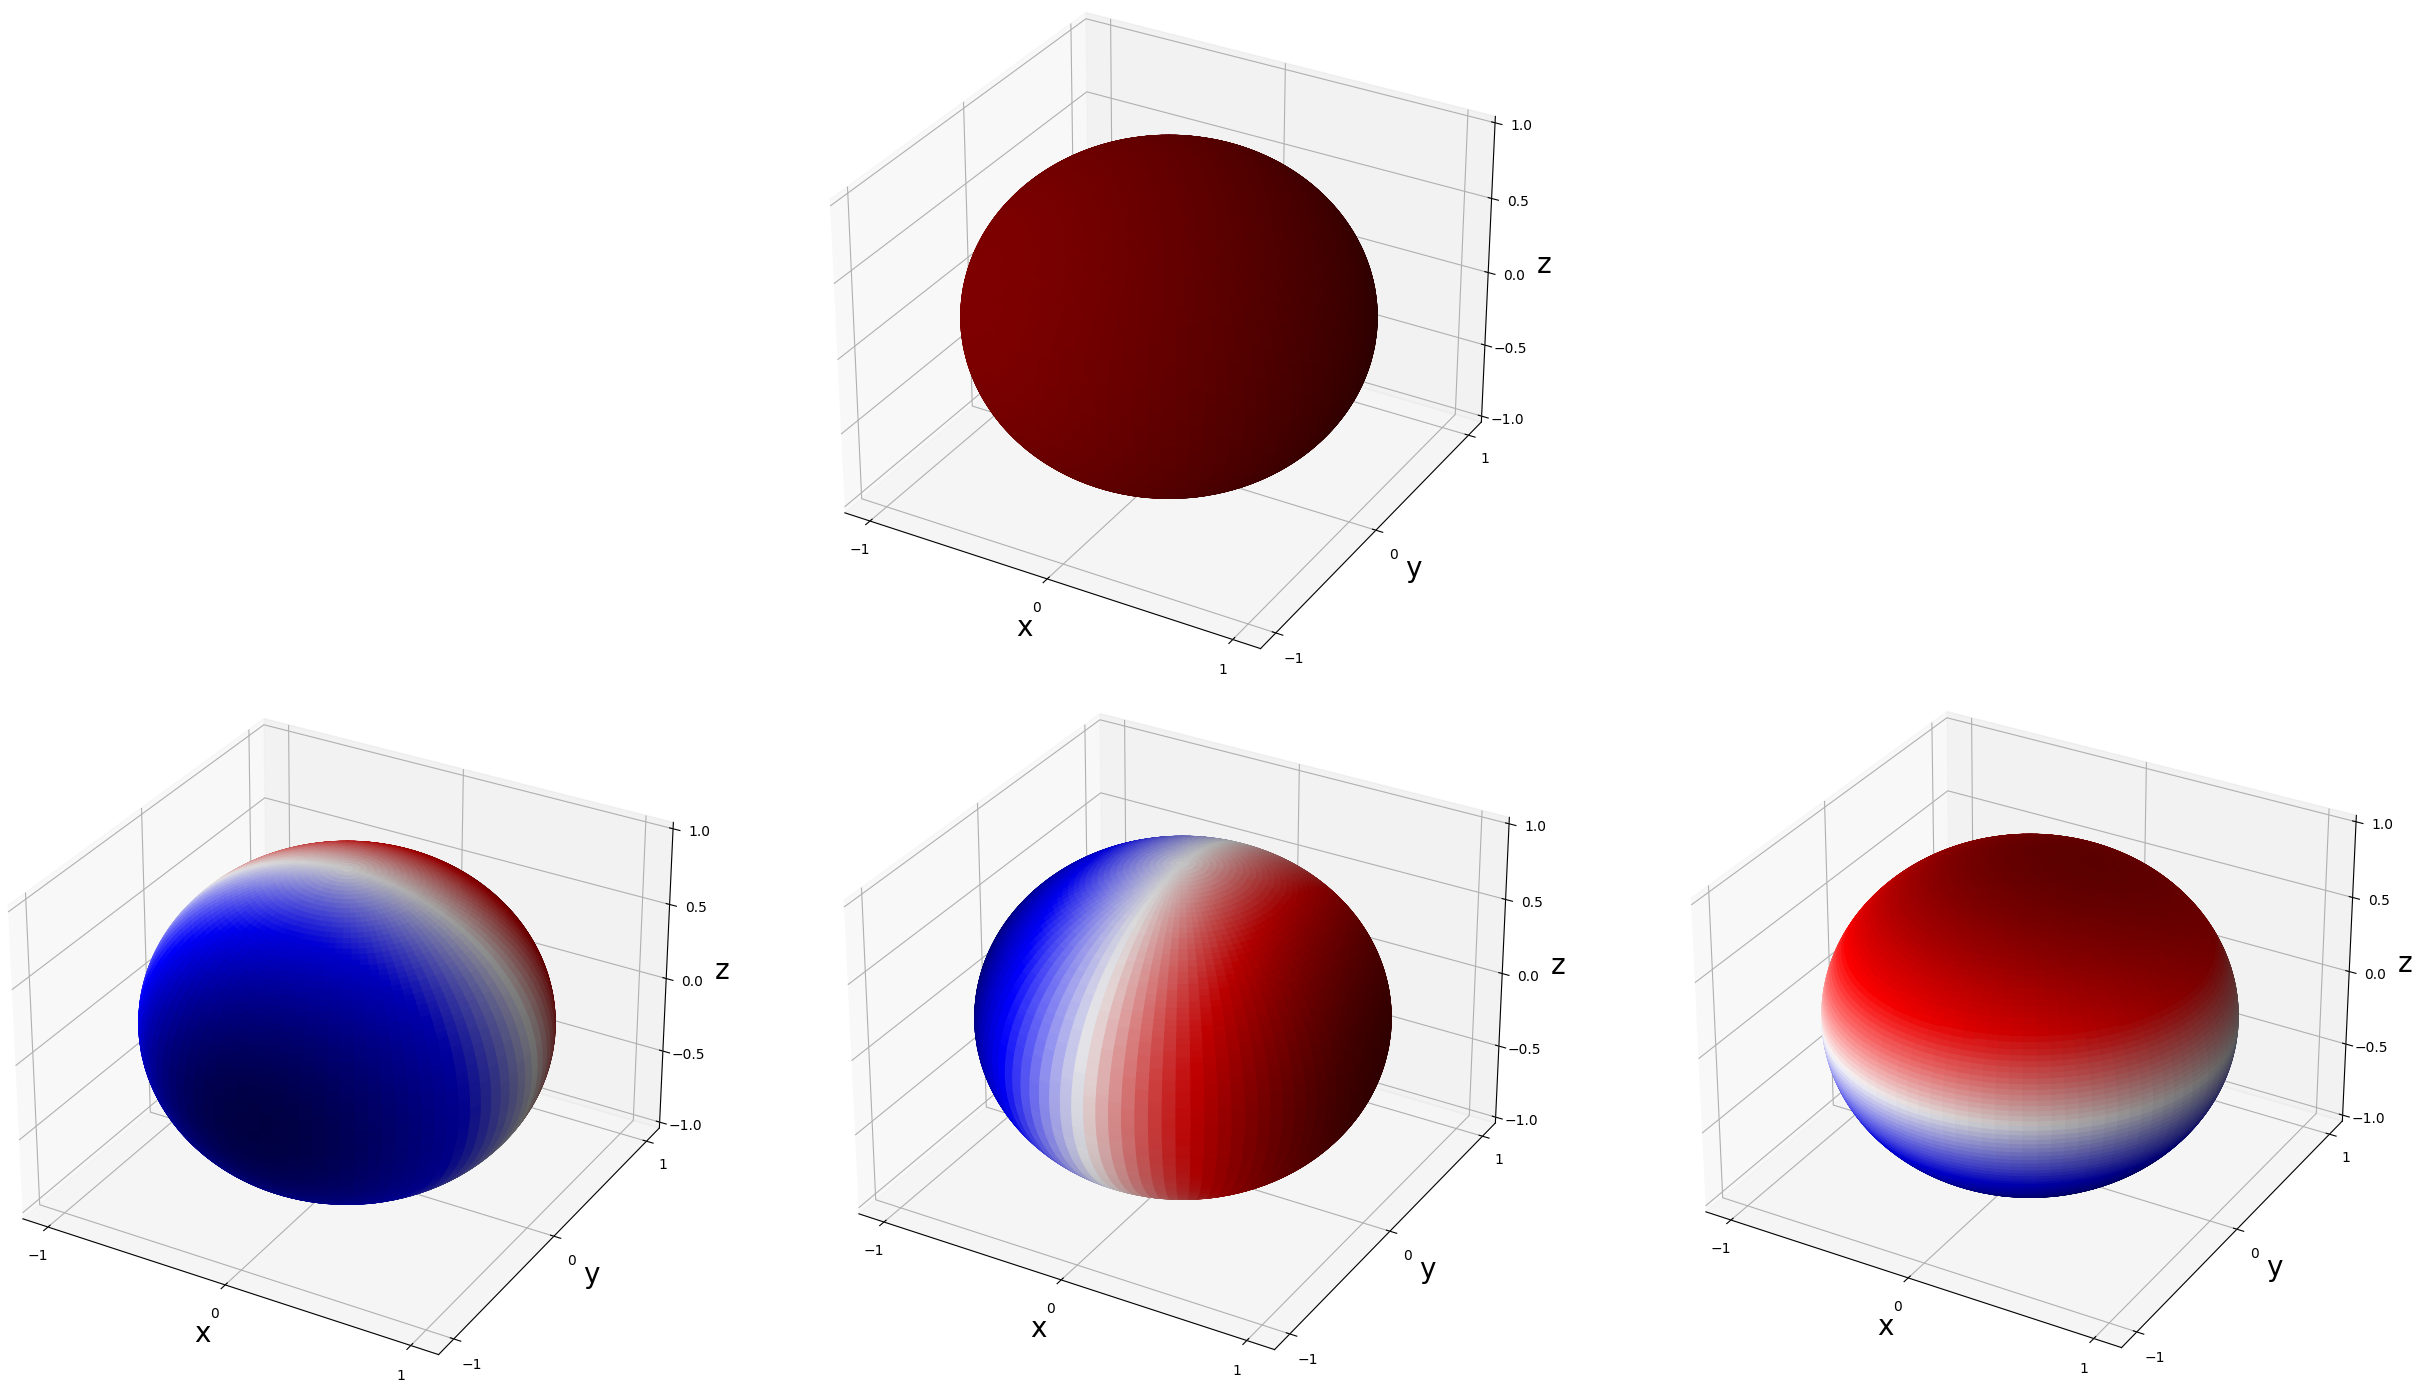
\includegraphics[width=1.\linewidth]{Images/chap2/foa.png}
    \captionof{figure}[First-order Ambisonics directivities]{First-order Ambisonics directivities. Top: $\tilde{Y}_0^0$ normalized, corresponding to $W$. Bottom, from left to right: $\tilde{Y}_1^1$, $\tilde{Y}_1^{-1}$, $\tilde{Y}_1^0$ normalized, corresponding to $X$, $Y$, $Z$, respectively. The red regions correspond to positive values and the blue regions correspond to negative values.}
    \label{fig:foa}
    \end{center}
\end{figure}

As a consequence of its low number of channels, which is a practical advantage here, the FOA format suffers from a low spatial resolution when representing the sound field \cite{rafaely_analysis_2005}. One consequence is the reduction of the \textit{sweet spot} size: it is the spatial region between the loudspeakers in which the restitution of the original sound field is the most accurate. 

Note that the Ambisonics format can be transposed directly into the short-time Fourier transform (STFT) domain, \emph{i.e.}, for each STFT time frame index $t$ and frequency bin $f$ \footnote{Note that in this thesis we use the notations $t$ and $f$ for the frame index and frequency bin in the STFT domain, as it is usually employed. Those notations are also used to express the physical frequency $f$ and time $t$ only for some preliminary discussions as in this chapter.}, we have:
\begin{equation}
\label{eq:foaSTFT}
\mathbf{x}(t,f) = 
\begin{bmatrix} W(t,f) \\ X(t,f) \\ Y(t,f) \\ Z(t,f) \end{bmatrix}
= \begin{bmatrix} 1 \\ \sqrt{3} \cos \theta_k \cos \phi_k \\ \sqrt{3} \sin \theta_k \cos \phi_k \\ \sqrt{3} \sin \phi_k \end{bmatrix} s(t,f).
\end{equation}

\subsection{Higher-order Ambisonics}

To improve the spatial resolution of the Ambisonics representation, we can increase the order $N$, leading to more components. When $N>1$, we call it the higher-order Ambisonics representation. For an order $N$, there are $(N+1)^2$ channels to represent the original signal. Table~\ref{tab:hoaComponents} sums up the directivities of the HOA components up to order 3, also illustrated in Fig~\ref{fig:hoa}. Using HOA components notably increases the size of the sweet spot and the resolution of the spatial characteristics of the encoded sound field, but at the cost of more channels to handle.

\begin{table}[h!]
\centering
\begin{tabular}{|cccc|}
\hline
$n$        & $m$ & \rule{0pt}{12pt} $\tilde{Y}_n^m$ & $\tilde{Y}_n^m(\theta,\phi)$ \\ \hline
   $0$               & \rule{0pt}{12pt} $0$           &  $\tilde{Y}_0^0$          & $1$           \\ \hline
\rule{0pt}{12pt}  & $-1$          &  $\tilde{Y}_1^{-1}$          & $\sqrt{3} \cos \theta \cos \phi$         \\
  $1$                &     \rule{0pt}{12pt} $0$      &   $\tilde{Y}_1^0$         &  $\sqrt{3} \sin \theta \cos \phi$    \\
                  &     \rule{0pt}{12pt}  $1$      &  $\tilde{Y}_1^1$          &       $\sqrt{3} \sin \phi$     \\ \hline
 & \rule{0pt}{14pt} $-2$        &  $\tilde{Y}_2^{-2}$          & $\frac{\sqrt{15}}{2} \sin 2 \theta \cos^2 \phi$           \\
                  &    \rule{0pt}{14pt} $-1$        &  $\tilde{Y}_2^{-1}$          &
                  $\frac{\sqrt{15}}{2} \sin \theta \sin 2 \phi$          \\
 $2$                 &  \rule{0pt}{14pt}   $0$       &  $\tilde{Y}_2^{0}$          &   $\frac{\sqrt{5}}{2} (3 \sin^2 \phi -1)$      \\
                  &   \rule{0pt}{14pt}  $1$       &  $\tilde{Y}_2^{1}$          &   $\frac{\sqrt{15}}{2} \cos \theta \sin 2 \phi$         \\
                  &   \rule{0pt}{14pt}  $2$       &  $\tilde{Y}_2^{2}$          &   $\frac{\sqrt{15}}{2} \cos 2 \theta \cos^2 \phi$         \\ \hline
 &  \rule{0pt}{14pt} $-3$            &  $\tilde{Y}_3^{-3}$          & $\sqrt{\frac{35}{8}} \sin 3 \theta \cos^3 \phi$            \\
                  & \rule{0pt}{14pt}  $-2$         &  $\tilde{Y}_3^{-2}$          & $\sqrt{\frac{105}{2}} \sin 2 \theta \sin \phi \cos^2 \phi$            \\
                  & \rule{0pt}{14pt} $-1$           &  $\tilde{Y}_3^{-1}$          & $\sqrt{\frac{21}{8}} \sin \theta \cos \phi (5\sin^2 \phi-1)$           \\
     $3$             &  \rule{0pt}{14pt} $0$         &  $\tilde{Y}_3^{0}$          &  $\frac{1}{2} \sin \phi (5 \sin^2 \phi -3)$          \\
                  &  \rule{0pt}{14pt}  $1$        &  $\tilde{Y}_3^{1}$          & $\sqrt{\frac{21}{8}} \cos \theta \cos \phi (5 \sin^2 \phi-1)$           \\
                  & \rule{0pt}{14pt} $2$           &  $\tilde{Y}_3^{2}$          & $\sqrt{\frac{105}{2}} \cos 2 \theta \sin \phi \cos^2 \phi$           \\
                  & \rule{0pt}{14pt} $3$           &  $\tilde{Y}_3^{3}$          & $\sqrt{\frac{35}{8}} \cos 3 \theta \cos^3 \phi$           \\ \hline
\end{tabular}
\caption[Directivities of HOA components]{Directivities of HOA components up to order 3, with the N3D normalization standard \cite{daniel_representation_2001}.}
\label{tab:hoaComponents}
\end{table}

\begin{figure}[t]
    \begin{center}
    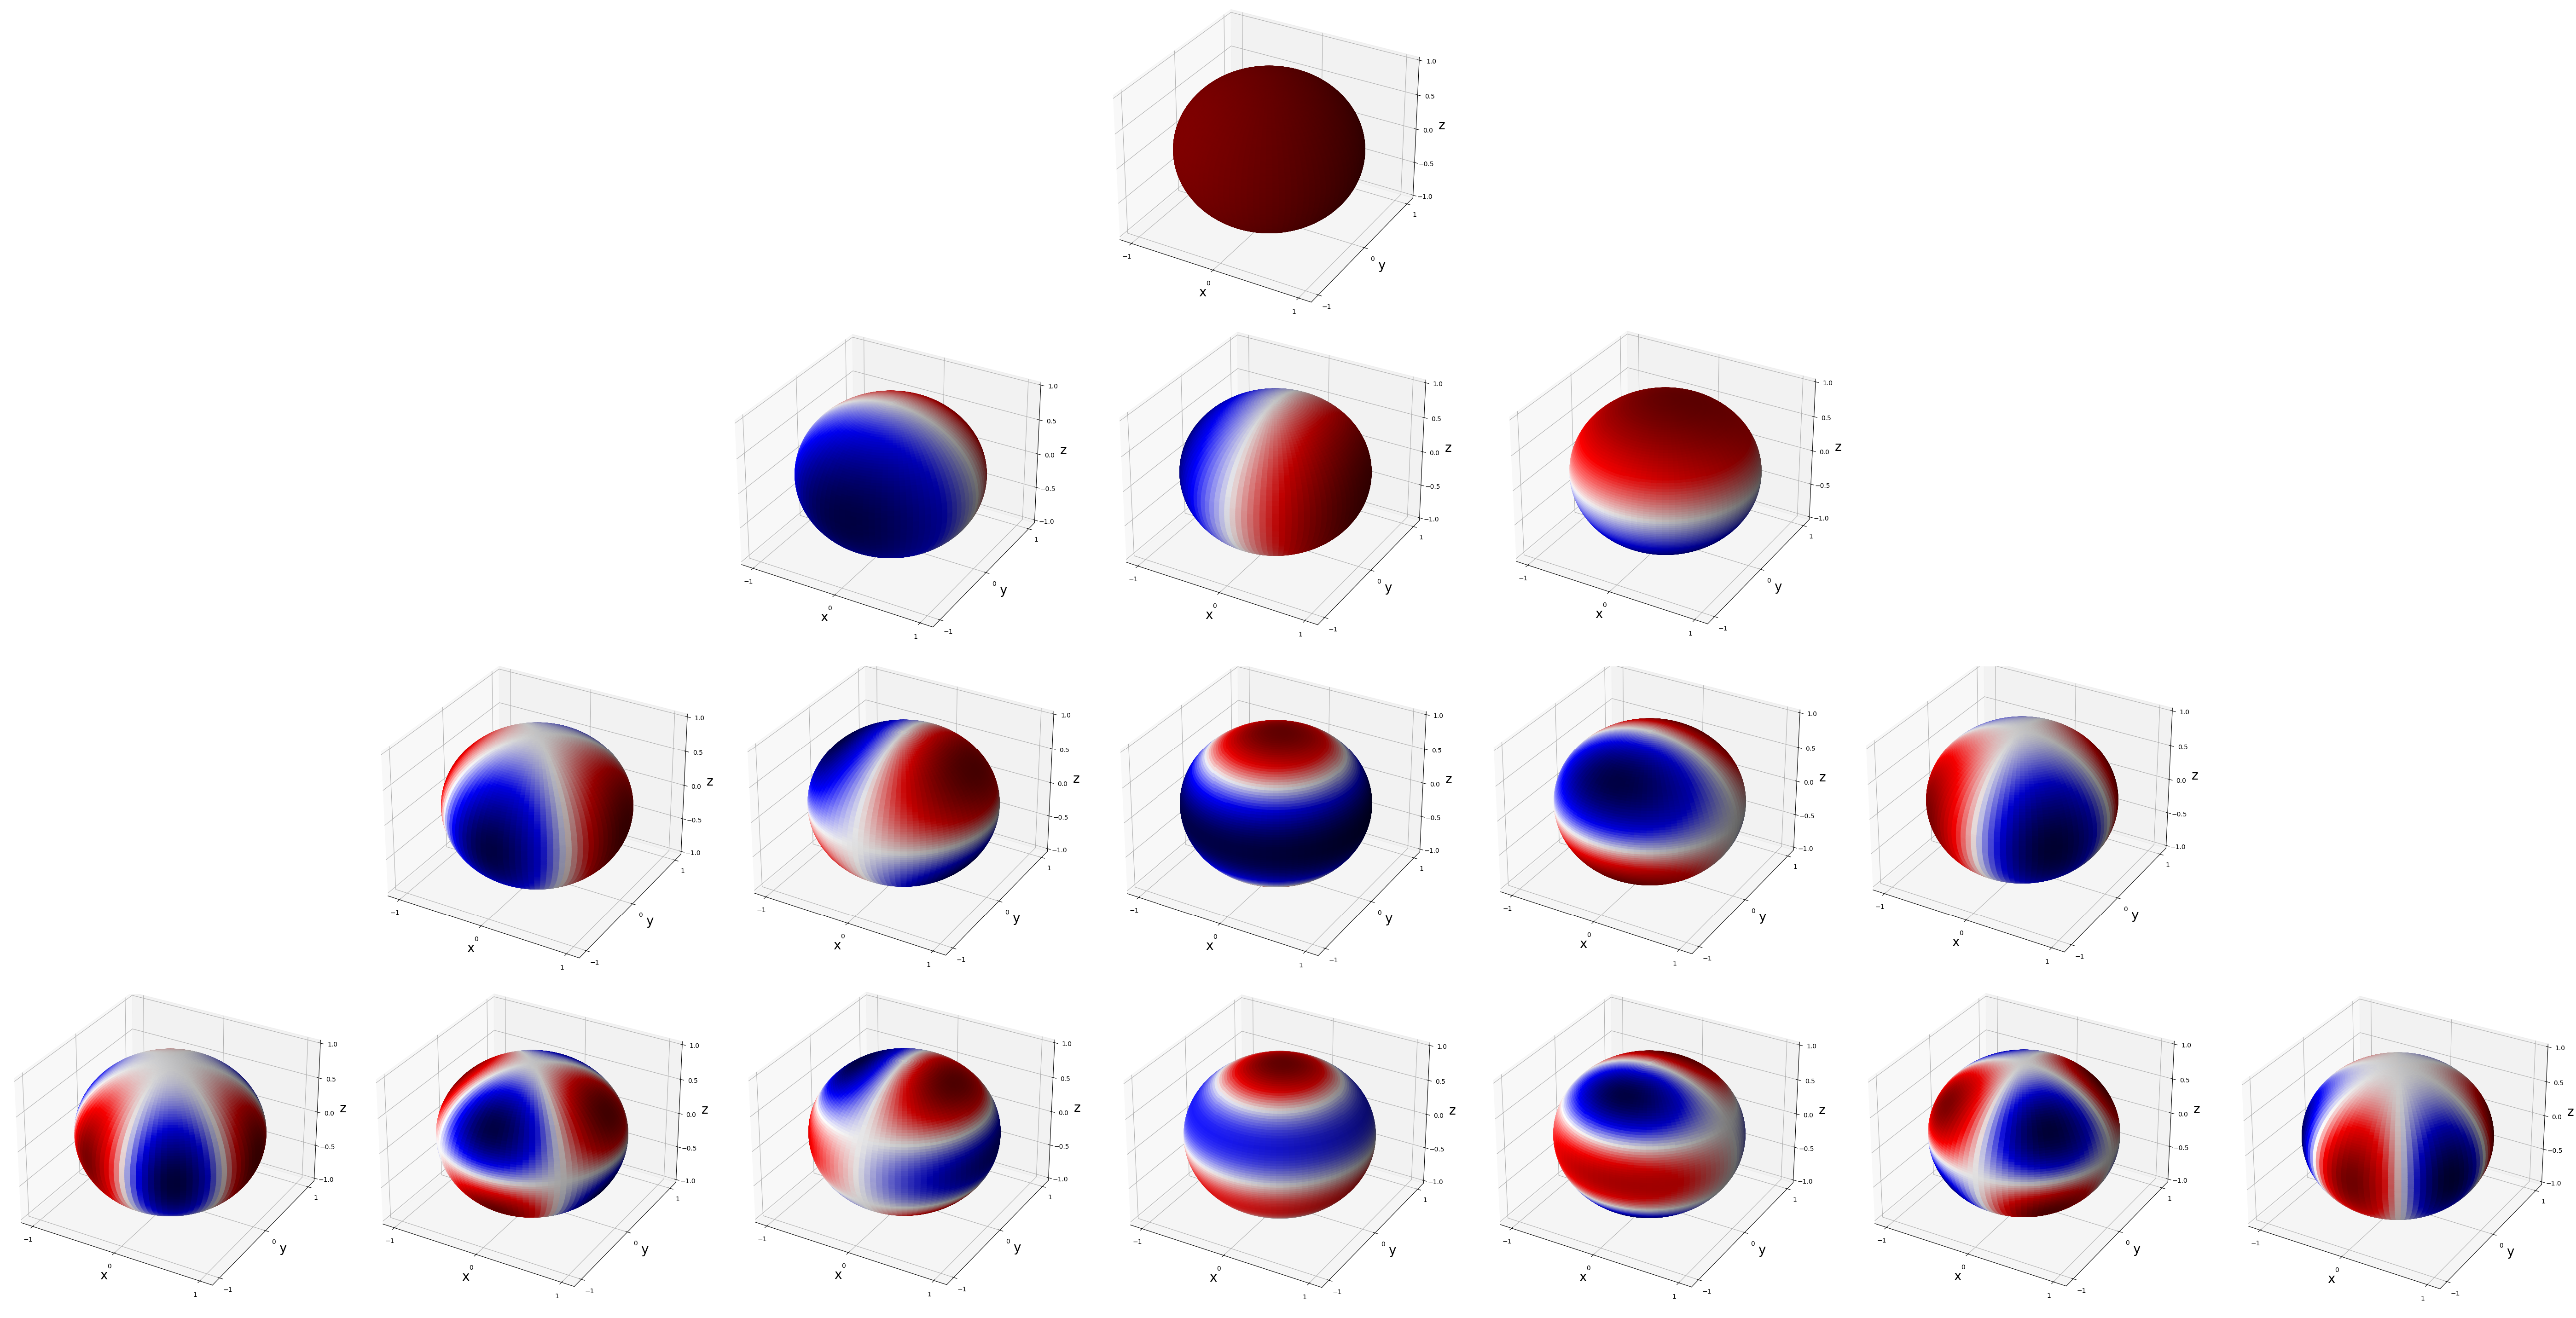
\includegraphics[width=1.\linewidth]{Images/chap2/hoa.png}
    \captionof{figure}[Higher-order Ambisonics directivities]{Higher-order Ambisonics directivities, with the spherical harmonics degree $n$ increasing from top to bottom and the order $m$ increasing from left to right. Red regions correspond to positive values and blue regions correspond to negative values.}
    \label{fig:hoa}
    \end{center}
\end{figure}


\subsection{Ambisonic encoding}
\label{subAmbEncoding}

In practice, Ambisonic signals (FOA or HOA respresentations) are computed from the finite number of acoustic pressure observations $\{p_i\}_{i\in[1,I]}$, measured by a microphone array. Denoting by $\mathbf{p} \in \mathbb{R}^I$ and $\mathbf{b} \in \mathbb{C}^{(N+1)^2}$ the vectors of concatenated observations $p(r,\theta_i,\phi_i,t)$, $i\in[1,I]$, and coefficients $B_n^m$, respectively, the expression~\eqref{eqAmbiDecomp} can be compactly written as
\begin{equation}
    \mathbf{p} \approx \mathbf{Y} \mathbf{W} \mathbf{b},
\end{equation}
where $\mathbf{Y} \in \mathbb{R}^{I \times (N+1)^2}$ is the matrix whose rows contain spherical harmonic functions $\tilde{Y}^m_n(\theta_k,\phi_k)$, evaluated at the directions $(\theta_i,\phi_i)$, and $\mathbf{W} \in \mathbb{C}^{(N+1)^2 \times (N+1)^2}$ is the diagonal weight matrix whose entries contain a sum of $i^n j_n(kr)$ and a regularization term \cite{nicol_sound_2010}. Without additional information, one would need a microphone array containing $I \geq (N+1)^2$ channels to obtain the coefficients $\mathbf{b}$ of the order $N$, which imposes practical limitation for the design of an Ambisonics microphone.

%-----------------------------------------------
%  INTENSITY, FDVV, TDVV
%-----------------------------------------------
\section{Sound intensity and velocity vector}

In the section~\ref{sec:ambisonics}, we introduced the definition of the Ambisonics coefficients, which are sufficient to entirely represent the sound field at any recording point. In this section, we present several representations based on the Ambisonics format which will be useful in the remainder of this thesis.

\subsection{Sound intensity vector}

\subsubsection{Definition}
\label{ss:pseudointensityVector}

Sound intensity is a fundamental acoustic quantity that is often used to characterize the distribution of energy of a sound field \cite{williams_fourier_2000}. Often expressed as a time-averaged quantity over certain temporal segment, it describes the magnitude and direction of the flow of sound energy per unit area \cite{jacobsen_fundamentals_2013}. For narrowband signals, one can define the complex ``steady state'' sound intensity vector as \cite{jacobsen_note_1991,williams_fourier_2000}:
\begin{equation}
\label{eq:intensityDefinition}
    \mathbf{I} = p \mathbf{u}^*,
\end{equation}
where $p$ is the sound pressure, $\mathbf{u}$ is the particle velocity vector, which is the physical velocity of the particles in motion which transmit the wave \cite{kinsler_fundamentals_2000}.

It can be shown that the sound pressure $p$ and the particle velocity vector $\mathbf{u}$ are related by the \textit{linearized fluid momentum equation} \cite[p.~27]{merimaa_analysis_2006}:
\begin{equation}
    - \nabla p = \rho_0 \frac{\partial \mathbf{u}}{\partial t},
\end{equation}
with $\nabla$ being the gradient operator and $\rho_0$ denoting the air density. 

The omnidirectional channel $W$ can be considered as an estimate of the acoustic pressure at the microphone position, while the FOA channels $X$, $Y$ and $Z$ approximate the spatial derivatives of pressure $p$ along the Cartesian coordinate axes \cite[p.~50]{merimaa_analysis_2006}. Therefore, one can approximate the particle velocity vector relatively to these channels with \cite[p.~90]{pulkki_parametric_2018} (the factor $1/\sqrt{3}$ is due to the presumed N3D normalization \cite{daniel_representation_2001}):
\begin{equation}
\label{eq:velocityVectorApprox}
\mathbf{u}(t) = - \frac{1}{\rho_0 c \sqrt{3}}
\begin{bmatrix} X(t) \\ Y(t) \\ Z(t) \end{bmatrix}.
\end{equation}
As we will see later, we are mainly interested in the \emph{direction} of the vector $\mathbf{u}(t)$, hence, by an abuse of notation, we also denote by $\mathbf{u}$ the normalized particle velocity vector. 

Since the previous equation is an approximation, injecting it into \eqref{eq:intensityDefinition} leads to an approximation of the intensity vector, which we call the \textit{pseudointensity} vector (PIV). To simplify the notation, we use the same symbol $\mathbf{I}$ to refer to the pseudointensity vector, which is now expressed using only the FOA components (in the STFT domain) as:
\begin{equation}
    \mathbf{I}(t,f) = \alpha \begin{bmatrix} W(t,f) X^*(t,f) \\ W(t,f) Y^*(t,f) \\ W(t,f) Z^*(t,f) \end{bmatrix},
\end{equation}
with $\alpha = - \frac{1}{\rho_0 c \sqrt{3}}$ a factor that will be dropped thereafter. As for the remaining of this thesis, we will refer to the pseudointensity vector based on FOA components as the \textit{first-order-pseudointensity vector} (FO-PIV).

\subsubsection{Active first-order-pseudointensity vector}

We define the \textit{active first-order-pseudointensity vector} as the real part of the complex FO-PIV:
\begin{equation}
    \label{eq:activeFOPIV}
    \mathbf{I}_a = \begin{bmatrix} \mathfrak{R}\big(W(t,f) X^*(t,f)\big) \\ \mathfrak{R}\big(W(t,f) Y^*(t,f)\big) \\ \mathfrak{R}\big(W(t,f) Z^*(t,f)\big) \end{bmatrix}.
\end{equation}
This quantity physically represents the transport of sound energy in the fluid, and it can be shown to be proportional to the gradient of the phase of sound pressure \cite{jacobsen_fundamentals_2013}. In other words, assuming free-field propagation, active intensity is orthogonal to the propagating wavefront.

\subsubsection{Reactive first-order-pseudointensity vector}

The \textit{reactive first-order-pseudointensity vector} is defined as the imaginary part of the complex FO-PIV:

\begin{equation}
\label{eq:reactiveFOPIV}
    \mathbf{I}_r = \begin{bmatrix} \mathfrak{I}\big(W(t,f) X^*(t,f)\big) \\ \mathfrak{I}\big(W(t,f) Y^*(t,f)\big) \\ \mathfrak{I}\big(W(t,f) Z^*(t,f)\big) \end{bmatrix}.
\end{equation}
Physically, the reactive FO-PIV represents the dissipative local energy transfers \cite{daniel_representation_2001}, and is orthogonal to the surfaces of equal energy of sound pressure \cite{jacobsen_fundamentals_2013,daniel_representation_2001}. While being negligible under the far/free field assumptions, reactive intensity becomes important in reverberant conditions.

\subsubsection{Higher-order pseudointensity vector}

We extend the previously introduced FO-PIV by using HOA components. The general expression for this \textit{higher-order-pseudointensity vector} (HO-PIV) is, at order $N$:
\begin{equation}
    \mathbf{I}^N(t,f) = B_0^0(t,f) \mathbf{B}_{1:N}^*(t,f),
\end{equation}
where $\mathbf{B}_{1:N}$ is the vector containing all HOA channels for $n=1$ to $N$ (there are $(N+1)^2-1$ channels in total). We can see that $\mathbf{I}^1$ corresponds to the FO-PIV. 

The definition of the active and reactive HO-PIV using HOA components ($\mathbf{I}^N_a$ and $\mathbf{I}^N_r$) is similar to the first-order case, \emph{i.e.}, they correspond to the real and imaginary part of the HO-PIV $\mathbf{I}^N$, respectively.

\subsubsection{Pseudointensity vector normalization}

A normalized version of the FO-PIV is obtained as follows:
\begin{equation}
     \bar{\mathbf{I}}(t,f) = \frac{\mathbf{I}(t,f)}{\lvert W(t,f) \rvert^2 + \frac{1}{3} \big(\lvert X(t,f) \rvert^2 + \lvert Y(t,f) \rvert^2 + \lvert Z(t,f) \rvert^2\big)}.
 \end{equation}
Note that the norm of $\bar{\mathbf{I}}(t,f)$ is upper bounded by $1$.

More generally, the normalized HO-PIV\footnote{Again, assuming the N3D normalization standard.} is given by:
\begin{equation}\label{eqHOpinv}
     \bar{\mathbf{I}}^N(t,f) = \frac{\mathbf{I}^N(t,f)}{\sum_{n=0}^N \frac{1}{2n+1} \sum_{m=-n}^n \lvert B_n^m \rvert ^2}.
\end{equation}

Assuming that the time-frequency bin $(t,f)$ is dominated by a single source, the normalized (FO-/HO-)PIV is independent of the source signal ``content'' $s(t,f)$, and mainly encodes the spatial footprint of sound propagation. This is easily observed for the plane wave propagation, since (according to \eqref{eqPlaneWaveCf}), we have $B_0^0 {B_n^m}^* \propto |B|^2$. The latter term cancels out in \eqref{eqHOpinv}, and the remaining part depends only on the corresponding spherical harmonics of different orders.

\subsection{Frequency-domain velocity vector}

The sound PIV was defined as the product between the first Ambisonics channel $W:=B_0^0$ and the other channels ($X$, $Y$ and $Z$ for FO-PIV, and all channels except $W$ for HO-PIV). We also showed a way to normalize the PIV to bound its values. A related representation, termed Frequency-Domain Velocity vector (FDVV) in  \cite{daniel_representation_2001}, is obtained by dividing the complex conjugate of FO-PIV by $\lvert W(t,f) \rvert ^2$:
\begin{equation}\label{eqFDVV}
    \mathbf{V}(t,f) = \frac{\mathbf{I}(t,f)^*}{\lvert W(t,f) \rvert ^2} = 
    \frac{1}{W(t,f)}
    \begin{bmatrix} X(t,f) \\ Y(t,f) \\ Z(t,f) \end{bmatrix}.
\end{equation}
Analogously to $\bar{\mathbf{I}}(t,f)$, due to the division by $\lvert W(t,f) \rvert ^2$, the FDVV has the advantage of being less dependent on the energy and therefore on the content of the signal. As for the complex PIV, we can separate the FDVV into the real and imaginary parts. 

\subsection{Time-domain velocity vector}
\label{ss:tdvv}

In this section, we will define the \textit{time-domain velocity vector} as the inverse Fourier transform (IFT) of the FDVV\footnote{Note that FDVV and TDVV are also known as \emph{Relative Transfer Function} and \emph{Relative Impulse Response} (in the spherical harmonic domain), respectively \cite{jarrett_theory_2017}.} \cite{daniel_time_2020}, but we modify the expression of the FDVV a bit beforehand.

We place ourselves in a single-source environment in which the Ambisonics recording captures the multipath signal. For a single timestep, due to the superposition principle \eqref{eqSRIR}, each recorded FOA channel will be a sum of delayed and attenuated copies of the source signal $s(t)$ (with an attenuation depending on the incoming wavefront direction and channel directivity). Under the far field assumption, the $n$\textsuperscript{th} such wavefront $\mathbf{x}_n(t)$ may be represented by a plane wave. According to \eqref{eqPlaneWave}, the FOA components of the plane wave propagating from the direction $(\theta_n,\phi_n)$, in frequency domain, are compactly expressed by
\begin{equation*}
    \mathbf{x}_n(f) = \left[ \begin{matrix} 1 \\ \sqrt{3} \mathbf{u}_n, \end{matrix} \right] s(f),
\end{equation*}
where $\mathbf{u}_n$ is the corresponding normalized particle velocity defined in \eqref{eq:velocityVectorApprox}.

The recorded signal, in the noiseless case, is then a sum of FOA-encoded plane waves:
\begin{equation*}
    \mathbf{x}(f) = s(f) \sum_{n} a_n(f) \mathbf{x}_n(f),
\end{equation*}
with $a_n(f)$ being the complex magnitude (incorporating both the common attenuation factor and phase shift) of the sound wave at frequency $f$.

Plugging these expressions into the definition of FDVV \eqref{eqFDVV}, we can now decompose the FDVV at frequency $f$ into the different reflections\footnote{Here we use the symbol ``$\simeq$'' instead of equality due to the N3D encoding factor $\sqrt{3}$ in the denominator. Without loss of generality, we drop this value in the ensuing expressions.}:
\begin{equation}
    \mathbf{V}(f) \simeq \frac{\sum_n a_n(f) \mathbf{u}_n}{\sum_n a_n(f)} = \frac{\mathbf{u}_0 + \sum_{n \geq 1} \gamma_n(f) \mathbf{u}_n}{1+\sum_{n \geq 1} \gamma_n(f)},
\end{equation}
where $\gamma_n(f) = \frac{a_n(f)}{a_0(f)} = g_n(f) e^{-2i \pi f \tau_n}$ is the relative \emph{gain} of the $n^{th}$ reflection with respect to the direct path (without losing generality we assume that $n$ follows the order of reflections).
Assuming that $\lvert \sum_{n \geq 1} \gamma_n(f) \rvert < 1$, we can express $\mathbf{V}(f)$ using the Taylor series of the function $f(x) = \frac{1}{1+x}$ :
\begin{equation}
    \mathbf{V}(f) = \Big(\mathbf{u}_0 + \sum_{n \geq 1} \gamma_n(f) \mathbf{u}_n \Big) \sum_{k=0}^{\infty} \Big( \sum_{n = 1}^{\infty} - \gamma_n(f) \Big)^k,
\end{equation}
which we can rearrange by separating the terms from the primary reflections and the terms coming from the interactions between reflections:
\begin{equation}
\begin{aligned}
        \mathbf{V}(f) &= \mathbf{u}_0 + \mathbf{u}_0 \sum_{k=1}^{\infty} \Big( \sum_{n=1}^{\infty} -g_n(f) e^{-2i \pi f \tau_n} \Big)^k \\
                      &+ \sum_{k=0}^{\infty} \sum_{n=1}^{\infty} \Big(g_n(f) e^{-2i \pi f \tau_n} \mathbf{u}_n \Big) \Big( \sum_{n=1}^{\infty} -g_n(f) e^{-2i \pi f \tau_n} \Big)^k \\
                      &= \mathbf{u}_0 + \mathbf{u}_0 \sum_{k=1}^{\infty} \sum_{n=1}^{\infty} \Big( -g_n(f) e^{-2i \pi f \tau_n} \Big)^k \\
                      &+ \sum_{k=0}^{\infty} \sum_{n=1}^{\infty} - \mathbf{u}_n  \Big( -g_n(f) e^{-2i \pi f \tau_n} \Big)^k + \Lambda(f),
\end{aligned}
\end{equation}
where $\Lambda(f)$ contains the cross terms of the interactions between reflections. Finally we obtain:
\begin{equation}
    \mathbf{V}(f) = \mathbf{u}_0 + \sum_{k=0}^{\infty} \sum_{n=1}^{\infty} \Big(\mathbf{u}_0 - \mathbf{u}_n \Big) \Big(-g_n(f)\Big)^k e^{-2i \pi f k \tau_n} + \Lambda(f).
\end{equation}

Assuming now that $g_n(f)=g_n$ is frequency-independent, we now apply the IFT of $\mathbf{V}$ to define the \textit{time-domain velocity vector} (TDVV) :
\begin{equation}
\label{eq:TDVVdefinition}
    \mathbf{V}(t) = \delta(t) \mathbf{u}_0 + \sum_{k=0}^{\infty} \sum_{n=1}^{\infty} \Big(\mathbf{u}_0 - \mathbf{u}_n\Big) (-g_n)^k \delta(t-k \tau_n) + \lambda(t),
\end{equation}
with $\delta$ denoting the Dirac delta function and $\lambda(t)$ the IFT of $\Lambda(f)$.

\begin{figure}[t]
    \begin{center}
    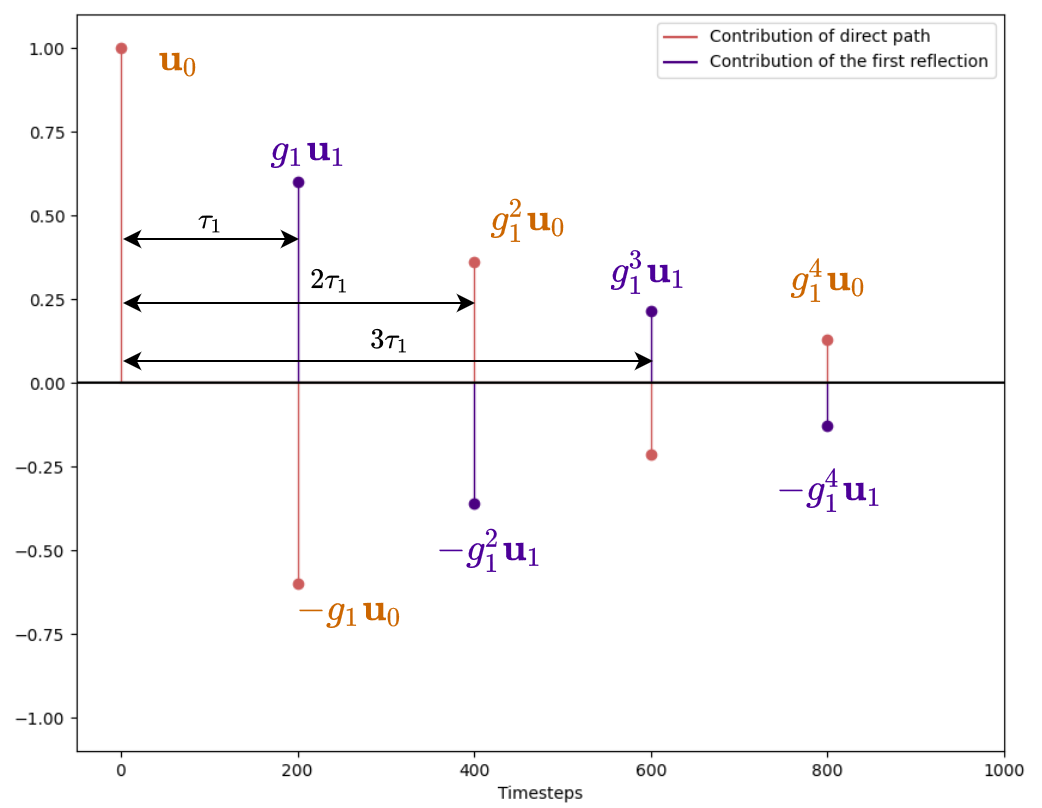
\includegraphics[width=0.8\linewidth]{Images/chap2/tdvv_1reflection_annote.png}
    \captionof{figure}[Theoretical time-domain velocity vector considering only one reflection]{Theoretical time-domain velocity vector considering only one reflection. The first orange peak at $t=0$ contains the coordinates of a vector colinear to the source DoA, representing the direct path between the source and the microphone array. The other orange peaks represent the contribution of the direct path to the value of the TDVV for different timesteps, while the purple peaks represent the contribution of the first reflection. All the peaks are equally spaced by an interval equal to $\tau_1$, and the peak amplitudes exponentially decay by a factor $-g_1$, with alternating sign.}
    \label{fig:TDVV_oneReflection}
    \end{center}
\end{figure}


In order to better appreciate the information contained in the TDVV, let us first assume that there is only one reflection in the considered environment:
\begin{equation}
    \mathbf{V}(t) = \delta(t) \mathbf{u}_0 + \sum_{k=0}^{\infty} \Big(\mathbf{u}_0 - \mathbf{u}_1\Big) (-g_1)^k \delta(t-k \tau_1) + \lambda(t).
\end{equation}
Fig.~\ref{fig:TDVV_oneReflection} illustrates what the TDVV looks like when considering only one reflection. As the TDVV is a vector with three coordinates (considering only the FOA domain), the coordinate in $y$-axis actually encodes the vector coordinates (the $x$-axis represents time). At $t=0$, we have $\mathbf{u}(0) = \mathbf{u}_0$ which is a vector colinear to the signal DoA. Then when $t$ increases we have a series of exponentially decaying peaks which are colinear to $\mathbf{u}_0 - \mathbf{u}_1$ at all time values which are multiples of $\tau_1$. Therefore we can theoretically retrieve the DoA, the first reflection direction, delay and relative gain with the TDVV under the assumptions of a single sound source with only one reflection and without noise.

\begin{figure}[t]
    \begin{center}
    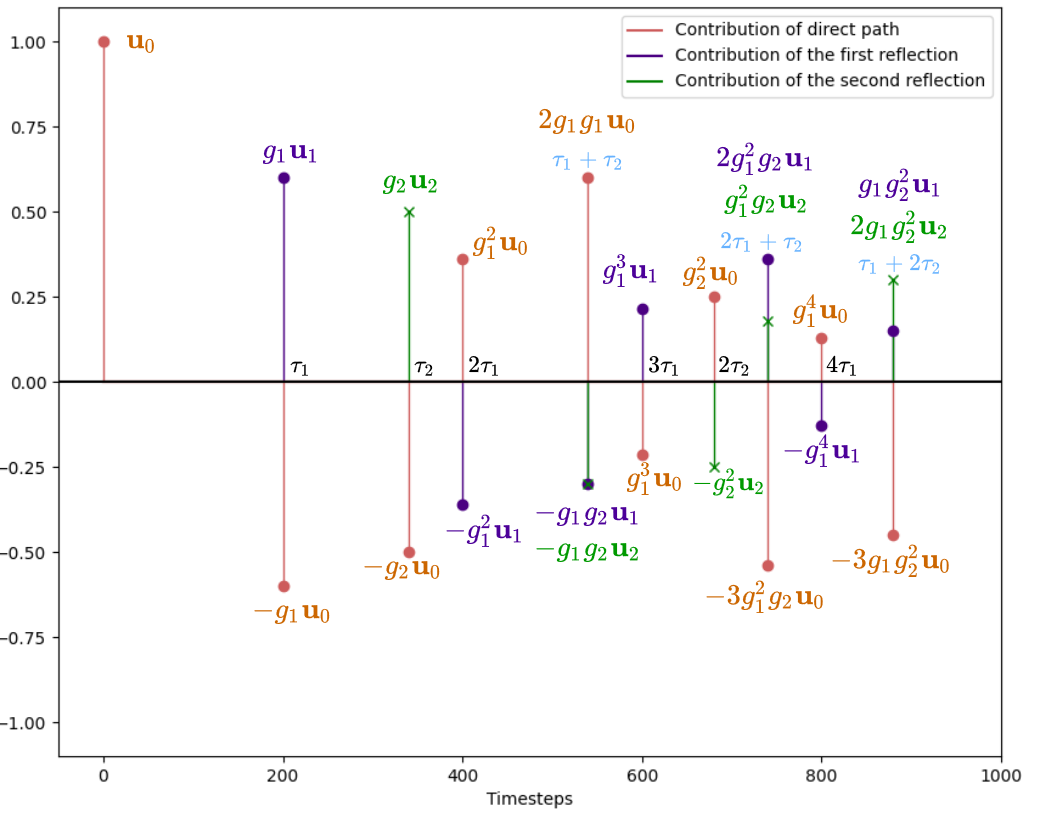
\includegraphics[width=0.8\linewidth]{Images/chap2/tdvv_2reflection_annote.png}
    \captionof{figure}[Theoretical time-domain velocity vector considering several reflections]{Theoretical time-domain velocity vector considering several reflections. The contributions of the direct path is represented in orange, those of the first reflection in purple and those of the second reflection in green. As in the case of only one reflection, the contributions corresponding to one reflection are equally spaced by $\tau_n$. In blue are indicated times for which the peaks contain the contributions of the interactions between the different reflections.}
    \label{fig:TDVV_twoReflections}
    \end{center}
\end{figure}

Now let us consider the general form of the TDVV with more than one reflection, leading to interaction between them. On Fig.~\ref{fig:TDVV_twoReflections} we can see what the TDVV looks like by illustrating the contributions of the direct path and the first two reflections, including the interactions (in blue in the figure). We can see that the peaks involving the contribution of only one of the reflections are still equally spaced by $\tau_n$. But now we see the appearance of some of the cross terms which were included in $\lambda(t)$ in \eqref{eq:TDVVdefinition}. Another phenomenon not represented in the figure can occur: theoretically, the different contributions of the reflections alone or those of the interaction between the reflections can overlap at the same time (related to the least common multiple of $\tau_n$) so it can be more difficult to separate the different contributions when analyzing the TDVV.

The TDVV thus provides an interesting representation to retrace the multipath propagation of a sound source. However, strong assumptions have been made to obtain an analytical expression for the TDVV: a single-source configuration without noise, frequency-independent gains, and the hypothesis that $\lvert \sum_{n \geq 1} \gamma_n(f) \rvert < 1, \forall f$ which is not fulfilled in practice. We do not push further the analysis of the TDVV in this thesis, since it is a relatively new idea in the literature. However, a certain number of experiments, discussed in Chapter~\ref{chap:tdvv}, has been conducted to exploit such a representation.


%-----------------------------------------------
%  CONCLUSION
%-----------------------------------------------
\section{Conclusion}

In this chapter, we introduced the framework we relied on in this thesis, based on the Ambisonics format. The main advantage of Ambisonics lies in the fact that it is capable of encoding a sound scene independently of the microphone array configuration, and without emphasizing any particular direction. We have shown the definition of the Ambisonics coefficients based on the spherical harmonics decomposition of the signal, which emerged from solving the wave equation in the spherical domain. These coefficients, considered at order $1$ (FOA) or higher (HOA), have been employed to define several physical quantities such as the FO- and HO-PIV, and the frequency-domain or time-domain velocity vector. All these sound representations have been used in our thesis work, generally as an input feature for neural networks, which are introduced in the next chapter.
